\chapter{Convolutional Neural Networks}
\label{sec:convnets}

While fully connected feed forward networks work well on data of
moderate dimensionality, training them becomes increasingly more
difficult once the number of inputs grows. In the case of image
classification for example, even an image with just a resulution of
256x256 pixels produces \(256 \cdot 256 = 65536\) inputs. Considering
that colored images usually have at least three color channels (take
the popular \textbf{R}ed \textbf{G}reen \textbf{B}lue color model as
an example), this multiplies the amount of input dimensions by a
factor of 3, yielding \(65536 \cdot 3 = 196608\) dimensions total. If
we wanted to use a fully connected hidden layer with only half as many
hidden neurons, we would have to optimize \(196608 \cdot 98304 =
19,327,352,832\) weights only for the first layer. Let us assume that
storing a weight in single precision floating point format
costs 4 bytes. This
would lead to spacial requirements of \(19,327,352,832 \cdot 4 =
77,309,411,328\) bytes or 77.31 gigabytes! One should quickly notice
that using this kind of neural networks to classify images is beyond
infeasible. But how is it possible that state-of-the-art classifiers
achieve human like performance in image classification, also
relying on artificial neural networks \cite{Russakovsky}? In the
following sections, we will explain how to modify our current feed
forward architecture in order to cope with these challenges and how
these astonishing results are possible.

\section{Overview}
\label{sec:conv-overview}

One characteristic of fully connected feed forward networks is that
every neuron in the first hidden layer is connected to every input
node. While this allows every neuron to make use of every piece of
information accross the whole input, it also increases the complexity
of the task that each neuron tries to solve. If the data has a
specific spatial structure, as would be the case for images, this
knowledge is not incorporated into the fully connected
architecture. In Convolutional Neural Networks (CNNs), the goal is to
reduce the model complexity by making use of the spacial structure of
the input. This is done by connecting each neuron of the first hidden
layer only to a locally constrained area of the image. We call this
area the \textit{local receptive field} of the neuron, see
Fig. \ref{fig:receptive-field}. Each neuron in
the first hidden layer will receive its own local receptive field of
inputs that it manages. This way, every hidden
neuron is no longer fully connected to every input, instead it is only connected to a
specific part of it. Looking at it
from a different perspective, the local receptive field acts like a
sliding window that is moved across the image, where each indermediate
position is represented by a hidden neuron. To reduce the complexity
of the model even further, every hidden neuron of a layer will share
its weights and biases with all the other neurons of that same layer,
drastically decreasing the amount of parameters. Intuitively, this
means that each neuron will look for the same input feature in the
data, the only difference being the local receptive field that each
individual neuron observes. This concept, also called a
\textit{convolution layer}, is the main foundation of the CNN
architecture \cite{Nielsen}.
\begin{figure}[h]
  \centering
  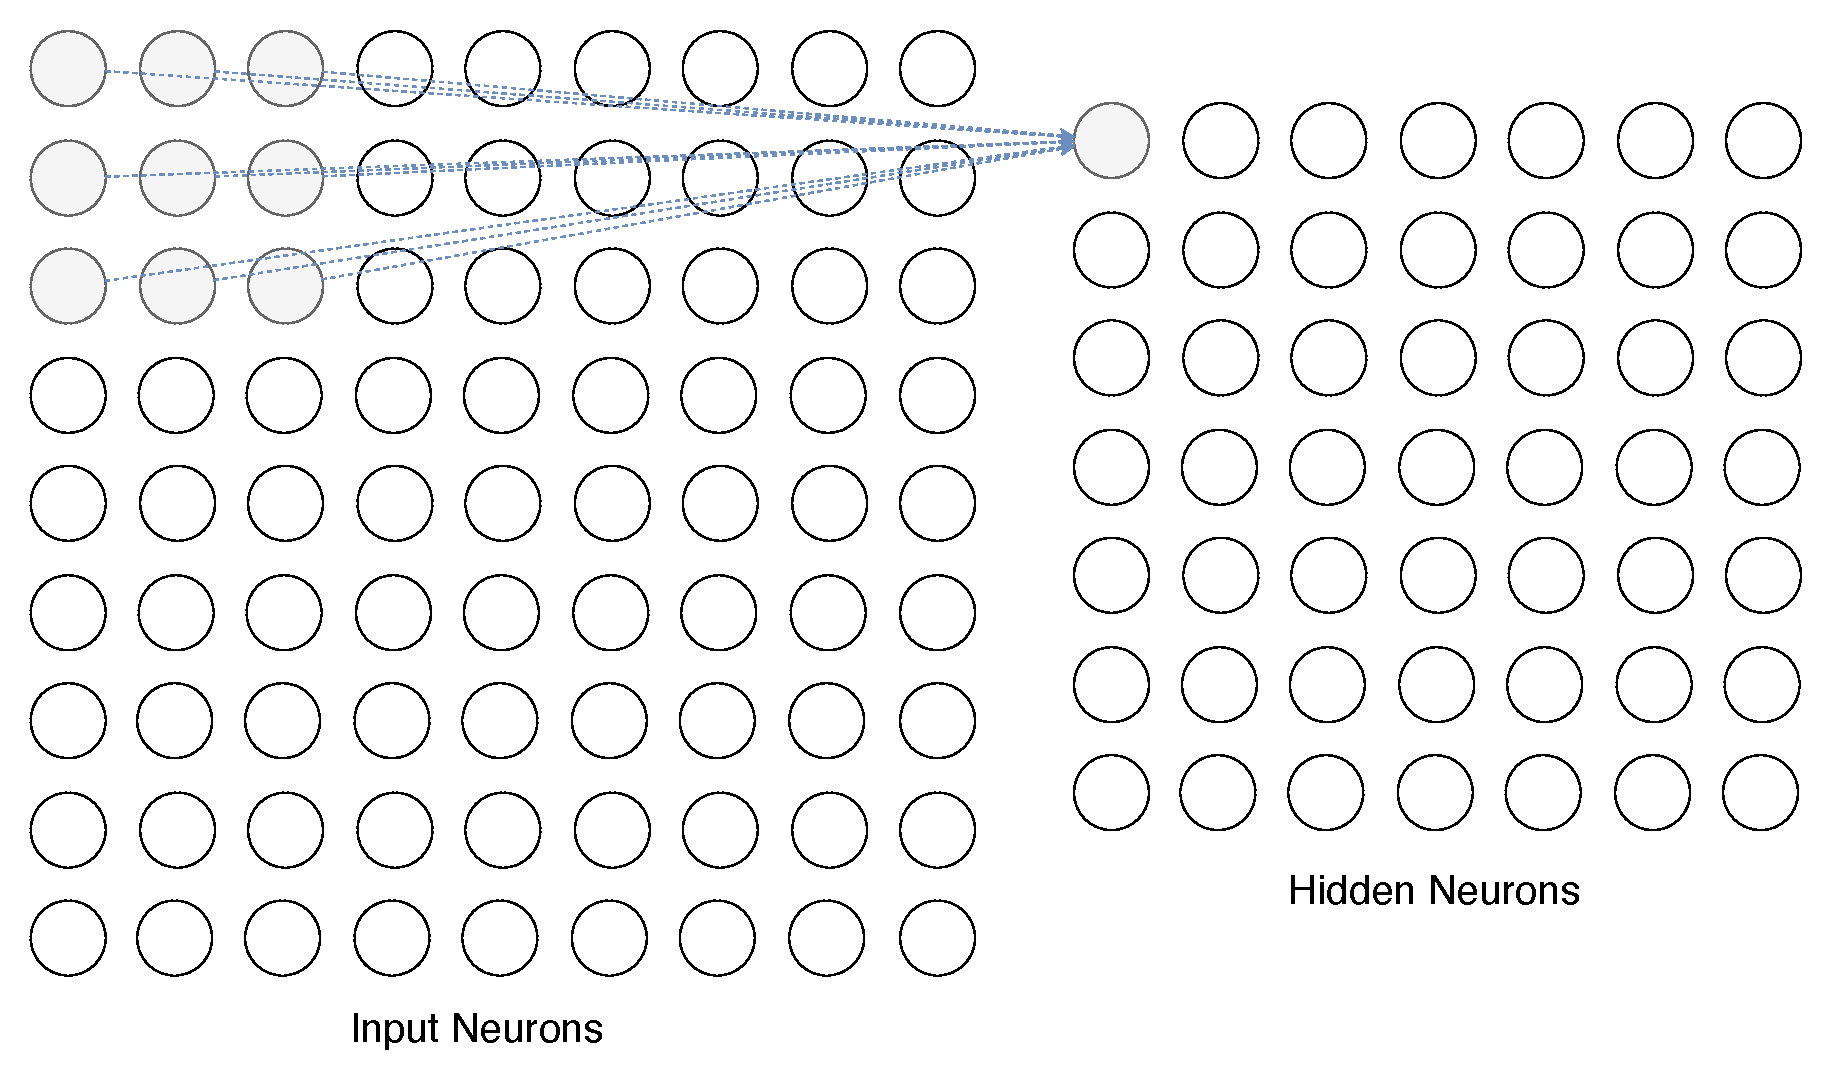
\includegraphics[width=\textwidth]{../figures/receptive_field}
  \caption{Illustration of the local receptive field of the first
    hidden neuron represented by the grey input units. The weights
    (depicted by the blue arrows) are shared among the hidden
    neurons.}
  \label{fig:receptive-field}
\end{figure}

\newpage
\section{The Convolutional Architecture}

The convolutional architecture is composed of three main parts
\cite{Patterson}\footnote{See \textit{CNN Architecture Overview} in
  chapter 4.}:
\begin{enumerate}
  \item The input layer
  \item Feature extraction layers
  \item Classification layers
\end{enumerate}
These components are stacked on top of each other to successively
break down the classification task into smaller problems, by first
extracting the relevant features from the data and then performing
classification on the basis of these high level features.
All the relevant layer types are described in
more detail within the following sections.

\subsection{The Input Layer}

Because CNNs are based on spatial assumptions on the input data, it
has to be arranged in a way that makes optimal use of its
structure. This is why it is most common to organize the input neurons
in the form of a two dimensional grid as shown in
Fig. \ref{fig:receptive-field}, where each cell resembles a
part of the input. In the case of image classification for example,
one would typically set the \(x\) and \(y\) dimensions of the grid
equal to the number of pixels in the input image in the corresponding
directions. This results in each input neuron in the grid resembling
one pixel in the image. If multiple input channels are present, one
would simply add a new layer of input neurons per channel, resulting
in a three dimensional arrangement. As was the case with ordinary feed
forward networks, the input layer does not compute an activation
function and just passes its signal further into the network.

\subsection{Feature Extraction Layers}

\subsubsection{Convolution Layers}

The convolution layer, which was briefly described above in section
\ref{sec:conv-overview}, is the main
component of the feature extraction block. It is used to detect
features across the input by having each neuron watch a specific part
of it. This can be visualized best by imagining the neurons be
arranged in a two dimensional grid where each neuron in the grid
watches a corresponding area in the input (see
Fig. \ref{fig:receptive-field}). To describe
this behaviour more precisely, we can slightly extend the neural model
we have already developed for feed forward networks (see section
\ref{sec:artificial-neurons}).

Recalling that the first component of the basic neural model was the
weighted sum of the inputs with a set of weights, we can transfer this
concept to convolutional layers by interpreting the weights as a
filter that each neuron applies to its local receptive field. This
filter, that we will also refer to as a kernel, can be described by a
stack of matrices of equal dimensions, where each matrix consists of
the weights that are applied to the local region in the input within
one channel. The amount of matrixes stacked corresponds to the depth
of the input data. When dealing with images, this would be the same as
the amount of channels (e.g. RGB has three color channels, thus the
kernel would consist of three stacked matrices). To compute the
weighted sum of the input with the filter, the dot product between the
local area of the input and the filter is applied and a bias value is
added as usual.

This procedure can also be expressed in terms of mathematical
equations as follows: Let the width of the kernel \(K\) be \(x_K\), the
height be \(y_K\) and the depth be \(d\), where \(d\) is usually equal
to the amount of different channels when dealing with images. Let us
further assume that the local receptive field of the current neuron
\(k\) can be described by the coordinates \((i, j)\) with respect to
the input \(X\), where \((i, j)\) indicates the shift of the field in
\(x\) and \(y\) direction. The result of applying the filter and
adding the bias value \(b\) can be denoted by the following formula:
\begin{equation}
  \label{Eq:convolution}
  z_k = \sum_{n=1}^{d}{\sum_{m=1}^{y_K}{\sum_{l=1}^{x_K}{X[i+l, j+m, n] \cdot
        K[l, m, n]}}} + b
\end{equation}
This operation is very similar to the concept of convolution in the
area of signal processing, which is the origin of the name
\textit{convolutional} neural networks.

After calculating the summation result \(z_k\) for every neuron in the
grid, an activation function is applied just like in feed forward
networks. Because of its various advantages, the most common choice is
the ReLU function (see section \ref{sec:relu}) which results in the
following expression describing the
output \(y_k\) of every neuron \(k\) in the grid:
\begin{equation}
  y_k = max(0, z_k)
\end{equation}
Carrying out this computation on every neuron in the
grid yields a new pattern of activations across the layer, which is
called a \textit{feature map} and can be interpreted intuitively as
follows: When computing the dot product between the kernel \(K\) and
the local receptive field of the neuron, this dot product acts like a
similarity measure between the local input and \(K\). When the dot
product is large, this indicates that the kernel and the local input
area very similar, when it is very negative, the input and the kernel
are contrasting. If the dot product is close to zero, this means that
kernel and input have almost nothing in common. Thus, areas of high
activity in the feature map indicate, where the input is most similar
to the kernel. Thinking further about this relationship, it follows
that the kernel \(K\) itself represents a \textit{feature} in the
input that every neuron watches out for, which is why the
convolutional layer is used as a \textit{feature extractor}.

To leverage this procedure even further, each convolution layer does
not only produce a single activation map for a single feature, but
repeats the process multiple times with different kernels, yielding a
stack of activation maps that display the presence of multiple
features. In addition to the amount of different features to detect,
there are a few other parameters to adjust in a convolution layer.
A brief overview of all these tunable parameters will be provided in
the following.

\paragraph{Kernel Size}

The kernel size can be described by the width and the height of each
neurons' local receptive field, see the grey input neurons in
Fig. \ref{fig:receptive-field}. In Eq. \ref{Eq:convolution}, these
dimensions are denoted by the parameters \(x_K\) and \(y_K\). Note that
the depth of the kernel is always predefined as the depth of the input
from the previous layer.

\paragraph{Kernel Stride}

This parameter defines how much the local receptive field is shifted
from one hidden neuron to the next. A stride of one in \(x\) and \(y\)
direction would indicate that the field is first shifted by one unit
along the \(x\) dimension and as soon as the end of the input is
reached, it would be reset to \(x=0\) and shifted one unit along the
\(y\) dimension, repeating the procedure. If the stride is smaller
than the size of the
kernel, the local receptive fields of the hidden neurons will overlap.
In Fig. \ref{fig:receptive-field}, there is a 7x7 grid of hidden
neurons which indicates that a stride of one in both dimensions was
used.

\paragraph{Number of Kernels}

This parameter describes the number of kernels to apply in a
convolution layer and, as we saw earlier, corresponds to the amount of
features to detect. Because every kernel results in its own feature
map, the depth of the output of a convolution layer is equal to its
number of kernels.

\subsubsection{Pooling Layers}
\label{sec:pooling}

Pooling layers are usually inserted after convolution layers to capture
the most essential patterns of the feature maps in order to reduce
their complexity. This is done by downsampling the activations,
resulting in a smaller input grid for the next layer. Quite similar to
convolution layers, a pooling layer can also be imagined as a filter
that runs over the input, but instead of computing dot products, this
filter only returns the maximum value of the region it is currently
looking at (see Fig. \ref{fig:pooling}). This technique is also known
as \textit{max-pooling}. It should be noted that there exist
alternative techniques such as average-pooling, where the average of a
region is computed and not the maximum, however max-pooling has proved
itself as the most effective pooling algorithm in practical
applications. Unlike convolution
layers, pooling layers do not influence the depth of the input
because each feature map is processed separately. There are two
parameters that can be adjusted in each pooling layer:
\begin{itemize}
  \item \textbf{Size:} This parameter controls the size of the filter
    that is used for downsampling.
  \item \textbf{Stride:} Similar to the stride parameter of a
    convolution layer, this value adjusts the step size in each
    direction that is taken during pooling.
\end{itemize}
Due to the fact that the downsampling operation purposefully discards
information regarding the exact location where the feature was
detected, this procedure contributes to the \textit{spatial
  invariance} of convolutional neural networks. What this means it that
the network is able to recognize certain features, no matter where
exactly they are located in the image. This is one of the most
important traits of the CNN architecture which greatly contributes to
its effectiveness in practical applications.

\begin{figure}[h]
  \centering
  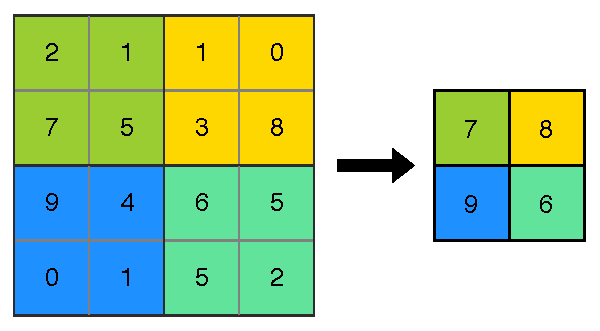
\includegraphics[width=0.5\textwidth]{../figures/pooling}
  \caption{Illustration of the max-pooling procedure on a single
    activation map. The filter size is \(2 \times 2\) and a stride of
    2 is used in each direction.}
  \label{fig:pooling}
\end{figure}

\subsection{Classification Layers}

After the feature extraction has been performed, the complexity of the
input data has usually been reduced significantly by stacking multiple
convolution and pooling layers. On the basis of this simpler and also
richer representation of the data, an ordinary fully connected feed
forward network can be used to perform the classification task. This
is done by inserting a fully connected hidden layer after the last
layer of the feature extraction part. This hidden layer is connected
to each neuron in the grid. Depending on the complexity of the
problem, it is also possible to insert multiple fully connected hidden
layers right after each other to complete the classification task. As
usual, the last layer consists of as many output neurons as there are
classes, employing the softmax activation function to compute the
classification result.

\section{Summary}

Putting all these layer types together typically results in a
convolutional architecture that is similar to what is displayed in
Fig. \ref{fig:convnet}. In this example, the convolution layers as
well as the pooling layers serve the purpose of feature extraction
while the fully connected network in the end is used to perform the
classification task based on the extracted features. Just as described
in the previous sections, the convolution layers usually yield
multiple feature maps while the pooling layers just downsample the
input they are presented with.

Similar to feed forward networks, these architectures can also be
trained using the gradient descent algorithm in combination with
backpropagation. During training, the weights and biases of each
layer, namely the different kernels for the convolution layers, are
adjusted in order to find a locally optimal configuration that suits
the classification task well.
\begin{figure}[h]
  \centering
  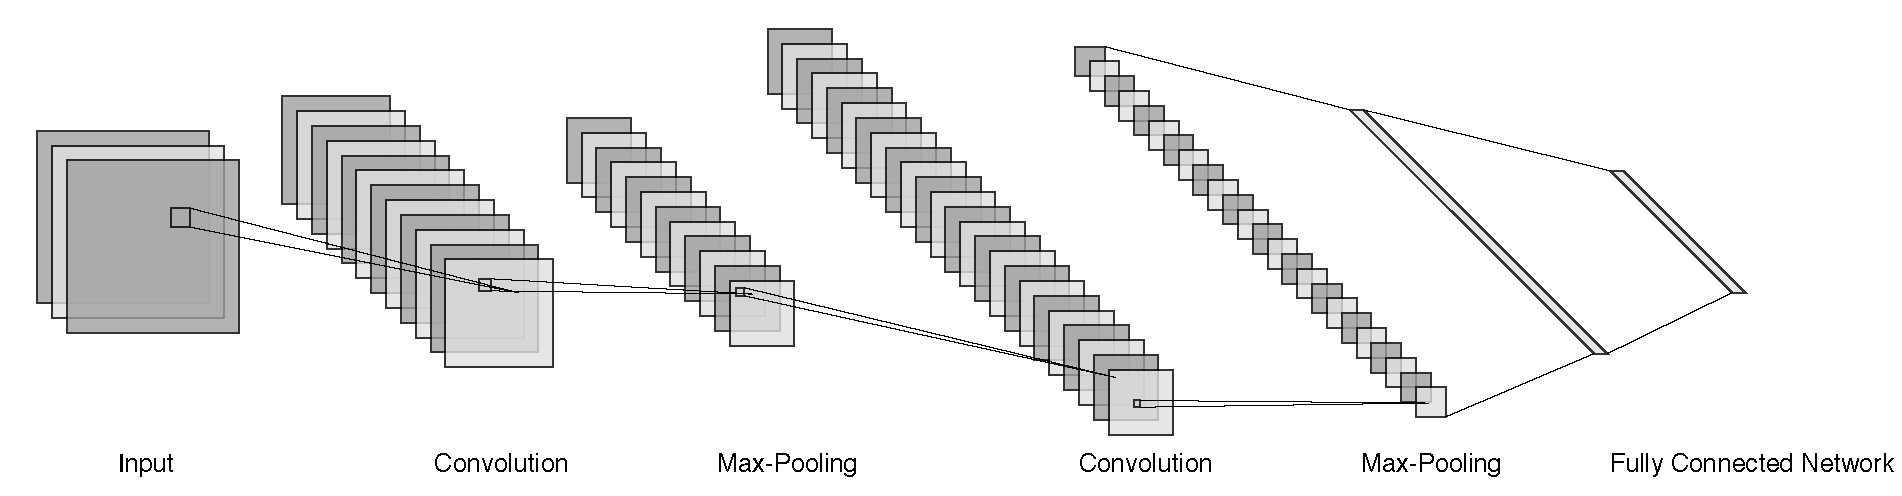
\includegraphics[width=\textwidth]{../figures/convnet}
  \caption{The typical architecture of a convolutional neural
    network.}
  \label{fig:convnet}
\end{figure}
